% !TEX root = writing_version.tex

\label{chp:theory}

\section{Hard sphere system}
\label{sec:HS_system}
The hard sphere system is the simplest model of a fluid going beyond the ideal gas only by including interactions between the single particles in the form of an occupied volume. Its well known potential between particles i and j is given in \autoref{eqn:hs_potential}.
\begin{equation}
\label{eqn:hs_potential}
V(r_{ij})=%\infty \cdot \Theta(\sigma - r_{ij})
\begin{cases}
\infty \quad & r_{ij} \le \sigma \\
0 \quad & r_{ij} > \sigma
\end{cases}
\end{equation}
In this equation $r_{ij} = r_j - r_i$ names the distance between the two particles and $\sigma$ is the diameter of the hard spheres.\\

While the ideal gas model without pair interactions already makes it possible to derive the famous equation of state $pV=NkT$, it does not include phase transitions yet. But these can be observed when granting the particles to occupy space in the simplest case by defining hard spheres of the kind in \autoref{eqn:hs_potential}. Because it is the simplest model and it is well feasible for computer simulations the hard sphere system is very well suited to study basic properties of first order phase transitions.\\ 

Compared to experiments where similar systems are possible, general properties of the system at hand can be varied very precisely without much effort and information about each single particle can be extracted easily as they are naturally required for the simulation.\\

On the downside computer simulations are much more constraint in their size, but with today's computational possibilities system of the order of 1 million particles become tractable, and such computer simulations become a powerful tool to study also phase transitions in simple systems.\\

The beginning of such simulations dates back to the beginning of electronic computer technology with first studies by Alder and Wainwright in 1959 \todo{cit the paper}. Since then more algorithms to increase efficiency have been elaborated, and technology advanced giving today the possibility of studying large scale systems. 

\section{The phase diagram and the meta stable fluid}
\label{sec:HS_phase_diagram}
The equation of state for the monodisperse hard sphere system has various approximations, \todo{cite an overview paper}. The most common approximation due to its simplicity is the Carnahan-Starling approximation
\begin{equation}
\label{eqn:CS}
Z=\frac{1+\eta+\eta^2-\eta^3}{(1-\eta)^3} \; \text{.}
\end{equation}
\todo{cite https://aip.scitation.org/doi/10.1063/1.1672048}
It approximates the compressibility factor Z depending on the packing fraction $\eta$ for the hard sphere fluid.\\

For the stable solid branch a common approximation is given by the Almarza equation of state \todo{cite https://aip.scitation.org/doi/full/10.1063/1.3133328}
\begin{equation}
\frac{p(v-v_0)}{k_B T} = 3 - 1.807846 y + 11.56350 y^2 + 141.6 y^3 - 2609.26 y^4 + 19328.09 y^5 \; \text{.}
\end{equation}
where p is the pressure, v is the volume per particle $v_0=\sigma^3/\sqrt{2}$ is the volume per particle at close packing, including the diameter of the spheres $\sigma$, and $y=p \sigma^3 / (k_B T)$, where $k_B$ is the Boltzmann constant and T is the temperature of the crystal.\\
Here the inverse of the volume per particle is the number of particles per volume $\rho = v^{-1}$. The relation to the corresponding packing fraction $\eta$ is given by $\rho = \frac{6}{ \pi} \eta$, which can be easily shown by extending $\rho = \frac{N}{V}$ by a single particles volume $V_s = \frac{4}{3} \pi \left(\frac{\sigma}{2}\right)^3 = \frac{\pi}{6} \sigma^3$.\\
Within the thesis mostly the volume fraction is used as it is the most common parameter for describing the system. Also the sphere diameter $\sigma$ is used as unit of length.\\ 

Returning to the phase diagram, the volume fraction for freezing has been determined to $\eta_{freeze} = 0.494$, the melting volume fraction has been calculated to be $\eta_{melt}=0.55$. In between these two both phases are in coexistence. This can be understood in the following way: The liquid may follow its branch to pressures above the coexistence pressure. But then it becomes more favourable for the particles to arrange into the crystalline phase as each single particle can access a larger free volume in the structured lattice than it would be possible in the unordered fluid.\\
By comparing the volume fractions of random close packing $\eta_{RCP}\approx 64\%$ with the one of a face centered cubic or hexagonal close packing fraction of $\eta_{HCP} \approx 74 \%$ this becomes clear. Within the crystalline phase each particle still has free volume accessible while the randomly packed particles are already confined at exactly one place.\\
The extra accessible volume translates into a larger number of possible states for the particle or in terms of thermodynamics a larger entropy, and such the metastable fluid will eventually find its equilibrium in the solid phase. As the solid phase will form with a volume fraction corresponding to $\eta_{melt}=0.55$ which is higher than the one of the metastable fluid, the pressure is mitigated and such not all fluid transforms into the solid phase, but both phases may coexist.\\
The overall phase diagram is shown with the constant coexistence pressure in \autoref{fig:hs_phase_diagram}.\\
\begin{figure}[h]
\centering
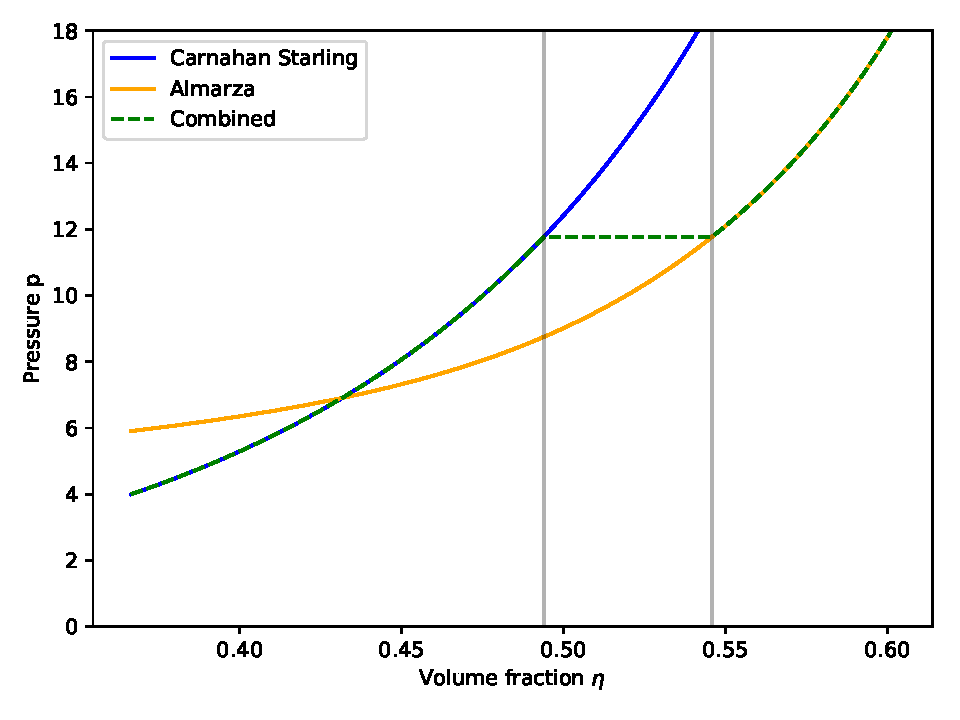
\includegraphics[width=0.6 \linewidth]{Hard_sphere_phase_diagram.pdf}
\caption{Phase diagram of the hard sphere system with freezing and melting volume fraction shown as shaded lines and the green dashed line indicating the equilibrium stable branch. Where liquid and solid branch do not coincide with the stable branch these are unstable and tend towards the stable branch.}
\label{fig:hs_phase_diagram}
\end{figure}





The solid fraction in terms of volume for the system $x_s = \frac{V_s}{V}$ with $V_s$ the solid volume and $V$ the total volume can be described within the coexistence region in the equilibrium state by \autoref{eqn:solid_fraction}.\\ 
For the derivation it is necessary to use that in the equilibrium state the density of the solid phase is given by the melting density and that the liquid density is equal to the freezing density, i.e $\rho_s = \rho_{melt}$ and $\rho_l = \rho_{freeze}$ respectively.\\
When further using the rather trivial equations
\begin{align}
V &= V_s + V_l \; \text{,} \nonumber\\
N &= n_s + n_l \; \text{,} \nonumber\\
N_i &= \rho_i V_i \; \text{,} 
\end{align}
with $n_{s/l}$ the number of solid/liquid particles we may write:
\begin{align}
\label{eqn:solid_fraction}
\rho V &= \rho_s V_s + \rho_l V_l \nonumber\\
\stackrel{\text{equil.}}{\Leftrightarrow} \quad \rho &= \rho_{melt} \frac{V_s}{V} + \rho_{freeze} \frac{V_l}{V} \nonumber \\
\Leftrightarrow \quad \rho &= \rho_{melt} \frac{V_s}{V} + \rho_{freeze} \frac{V - V_s}{V} \nonumber \\
\Leftrightarrow \rho &= \rho_{melt} \frac{V_s}{V} + \rho_{freeze} \left( 1- \frac{V_s}{V} \right) \nonumber \\
\Leftrightarrow \frac{V_s}{V} &= \frac{\rho - \rho_{freeze}}{\rho_{melt} - \rho_{freeze} } 
\end{align}
As the solid fraction below $\rho_{freeze} $ vanishes and above $\rho_{melt}$ is 1, we can conclude that the equilibrium solid fraction of the system is given by \autoref{eqn:solid_fraction_result}.
\begin{align}
\label{eqn:solid_fraction_result}
x_s(\rho) = 
\begin{cases}
0 & \rho <  \rho_{freeze}\\
\frac{\rho-\rho_{freeze}}{\rho_{melt}-\rho_{freeze}} &  \rho_{freeze} < \rho <  \rho_{melt}\\ 
1 &  \rho > \rho_{melt} \quad \quad \text{.}
\end{cases}
\end{align}

%\begin{align}
%\label{eqn:solid_fraction}
%N \rho &= n_s \rho_s + n_l \rho_l \nonumber\\
%\Leftrightarrow \quad \rho &= \frac{n_s}{N} \rho_s + \frac{N-n_s}{N} \rho_l \nonumber\\
%\Leftrightarrow \quad \rho &= x_s \rho_s + (1-x_s) \rho_l \nonumber\\
%\Leftrightarrow \quad x_s &= \frac{\rho-\rho_l}{\rho_s-\rho_l} \; \text{,}
%\end{align} 
%where further $n_l = N - n_s$ is the number of liquid particles. As the solid fraction below $%\eta_{freeze} $ vanishes and above $\eta_{solid}$ is 1, we can conclude that the equilibrium solid %fraction of the system is given by \autoref{eqn:solid_fraction_result}.
%\begin{align}
%\label{eqn:solid_fraction_result}
%x_s(\rho) = 
%\begin{cases}
%0 & \rho <  \rho_l\\
%\frac{\rho-\rho_l}{\rho_s-\rho_l} &  \rho_l < \rho <  \rho_s\\ 
%1 &  \rho > \rho_s \quad \quad \text{.}
%\end{cases}
%\end{align}


Evaluating the above result at feasible volume fractions for nucleation in between $\eta \in [0.53,0.55]$ leads to coexistence fractions of $x_s \in [0.7,1]$. This means that we are expecting large parts of the system to be in the solid phase after long waiting times.\\

As pointed out earlier the phase transition takes place as it reduces the pressure in the liquid. This means that already during the growth of clusters the volume fraction of the metastable liquid is reduced, potentially altering its behaviour significantly. For closer inspection of this the particle density of the metastable liquid depending on the solid fraction $x_s$ is evaluated in \autoref{eqn:meta_stable_volume_fraction}. For this purpose first the liquid volume $V_l$ and the number of liquid particles $N_l$ is expressed in terms of the solid fraction $x_s$:
\begin{align}
V_l(x_s) & = V(1-x_s)\\
N_l(x_s) & = N-n_s(x_s) = N - \rho_m V x_s = N(1-\frac{\rho_m}{\rho}x_s)
\end{align}
Following it is combined with the result:
\begin{align}
\label{eqn:meta_stable_volume_fraction}
\rho_l(x_s) &= \frac{N_l (x_s) }{ V_l(x_s) } = \frac{N}{V} \frac{1-\frac{\rho_m}{\rho}x_s}{1-x_s} = \rho \frac{1-\frac{\rho_m}{\rho}x_s}{1-x_s}
\end{align}
Some examples of \autoref{eqn:meta_stable_volume_fraction} are depicted in \autoref{fig:remaining_density} for moderate solid fractions of the system at regular volume fractions used for nucleation.\\
\begin{figure}[h]
\centering
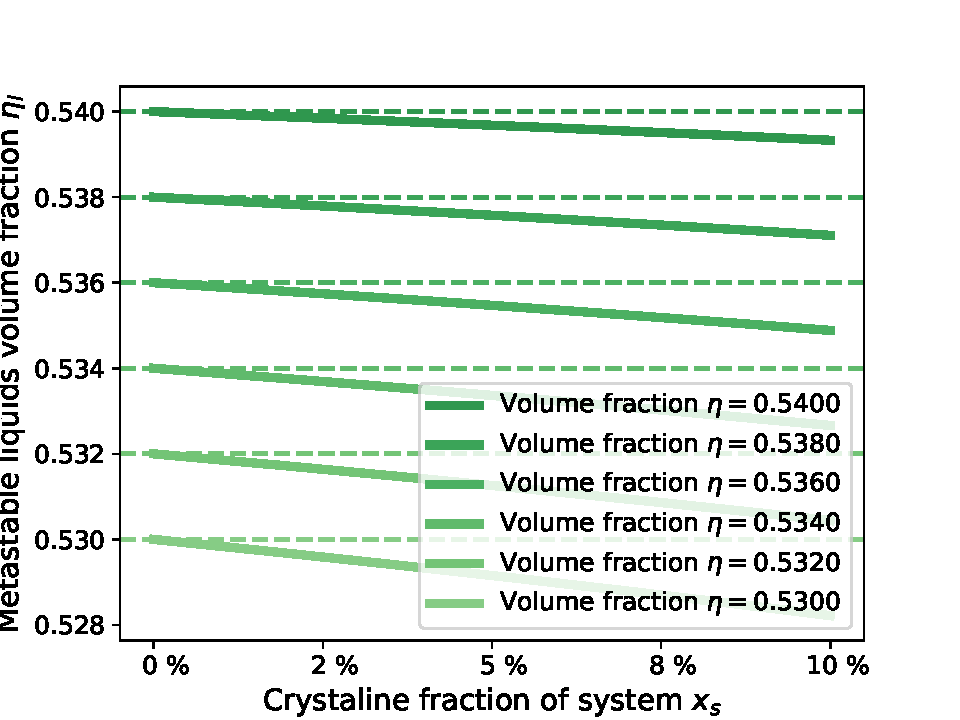
\includegraphics[width=0.7 \linewidth]{remaining_density.pdf}
\caption{Visualization of \autoref{eqn:meta_stable_volume_fraction}. The volume fraction of the remaining liquid decreases for all shown initial volume fractions only little up to crystalline ratios of a few percent.}
\label{fig:remaining_density}
\end{figure}
What can be seen is that for crystalline fractions of a few percent the remaining liquid is not altered significantly. Especially for system sizes of about 1 million particles it corresponds to cluster sizes of a few ten thousand particles, where stable growth of clusters takes place which is rather insensitive to changes of the volume fraction as shown in \autoref{sec:cluster_growth}. This means that during the highly sensitive cluster forming processes the volume fraction of the liquid can be assumed to be stable.\\ 

%Eventhough not further discussed in this thesis it might be said that for polydisperse radii the phase diagram becomes even richer as show for example in 
%\todo{https://journals.aps.org/prl/pdf/10.1103/PhysRevLett.91.068301}

\section{Classical nucleation theory }
\label{sec:CNT}
Classical nucleation theory (CNT) has been proposed \todo{look who did this the first time} and since then multiple times modified to describe various types of systems to account for deviations off experimental results \todo{look if tanja cited someone else here}. Still it provides some reference  or expectation to compare with the simulation data.\\

CNT assumes that a spherical crystallite may form in the liquid with properties of the bulk crystal while the fluid remains with the properties of the bulk liquid. The difference in the free energy landscape is given by a surface and a volume term. The first arises from the surface tension $\gamma$ between the fluid bulk and solid bulk phases. The second comes by the difference in chemical potential $\Delta \mu$. The whole expression reads:
\begin{equation}
\label{eqn:free_energy}
\beta \Delta G(R) =4 \pi R \gamma -\frac{4}{3} \pi R^3 \rho \Delta \mu  
\end{equation}
Where $\rho$ is the particle density of the solid phase.\\

For the difference of the chemical potential $\Delta \mu $ we use the free energy difference between the metastable liquid branch and the stable coexistence branch. To calculate it we employ the differential relation of the free energy
\begin{align}
\label{eqn:differential_relation}
dF = -S  \, dT -P \, dV + \mu  \, dN
\end{align}
at a constant number of particles and constant temperature. By further reformulating $dV$ by using $ dN = dV  \, \rho + V  \, d\rho  $ and $dN = 0 $ we find  $ dV = -d\rho \frac{N}{\rho^2}$. With it \autoref{eqn:differential_relation} becomes
\begin{align}
\label{eqn:df_relation}
\frac{dF}{N} = \frac{P(\rho)}{\rho^2} d\rho \; \text{.}
\end{align}

The pressure $p(\rho)$ is given by the equation of state and approximated by the Carnahan-Starling approximation \autoref{eqn:CS} where $\eta = \frac{6 \rho }{\pi}$ and $Z=\frac{pV}{NkT} = \frac{p(\rho)}{\rho kT}$. Integrating \autoref{eqn:df_relation} between two densities leads to
\begin{equation}
\frac{\Delta F}{N} = \int_{\rho_1}^{\rho^2} \frac{kT}{\rho} \frac{1+\left( \frac{6 \rho}{\pi}\right) +\left( \frac{6 \rho}{\pi}\right)^2 - \left( \frac{6 \rho}{\pi}\right)^3}{\left( 1 - \frac{6 \rho}{\pi}\right)^3} d\rho
\end{equation}
which has the analytical solution:
\begin{equation}
\int_{x_1}^{x_2} \frac{1+(ax) +(ax)^2 - (ax)^3 }{( 1 - ax )^3 x} dx = \left. \frac{3-2ax}{(ax-1)^2} + \text{log}(x) \right|_{x=x_1}^{x_2}
\end{equation}
further omitting the lengthy notation for $\eta = \left( \frac{6 \rho}{\pi}\right)$ we end up with
\begin{equation}
\frac{\Delta F}{N} = kT \left(  \frac{3-2 \eta_2}{(\eta_2 - 1)^2} - \frac{3-2 \eta_1}{(\eta_1 - 1)^2} + \text{log}\left( \frac{\eta_2}{\eta_1} \right) \right)
\end{equation}
The analytical solution is compared in \autoref{fig:free_energy_diff} with numerically found results which have been calculated before the analytical solution was found. The difference in free energy is in the following identified with the difference in chemical potential $\Delta \mu$. \\

\begin{figure}[h]
\centering
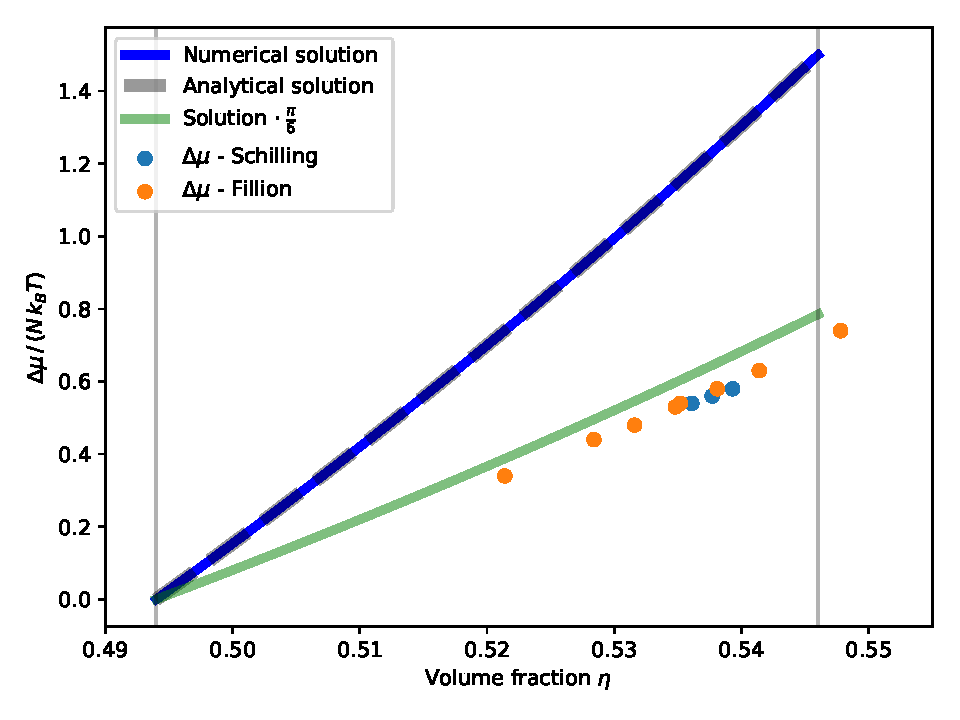
\includegraphics[width=0.7 \linewidth]{Free_energy_difference.pdf}
\caption{Free energy difference per particle between the metastable liquid phase and the coexistence phase. Values found in the literature deviate from the shown result, but it is speculated that a factor of $\frac{\pi}{6}$ common in the calculations is missing in either this or their calculation, as the modified green curve collapses rather accurately on the literature values when choosing $\eta_{freeze}=0.5$.}
\label{fig:free_energy_diff}
\end{figure}


Coming back to the free energy landscape of \autoref{eqn:free_energy} we see that it exhibits a maximum at a radius called $R_{crit}$. The interpretation of this radius is that if a cluster surpasses the critical radius it is likely to continue to grow until it incorporates all available fluid. Cluster in this sense is defined as a structure having a crystalline like ordering locally. The critical radius is given by \autoref{eqn:r_crit}.

\begin{equation}
\label{eqn:r_crit}
R_{crit} = \frac{2 \gamma}{\rho \Delta \mu }
\end{equation}

Furthermore the height of this barrier can be calculated by common algebra to be 
\begin{equation}
\beta \Delta G (R_{crit}) = \frac{16 \pi \gamma^3}{3 \rho^2 (\Delta \mu )^2}
\end{equation}

The classical calculated critical radius depending on the volume fraction is depicted in \autoref{fig:r_crit} for an first impression of the cluster sizes that we are expecting for nucleation. The value of the surface tension is set to $\gamma = 0.6$. \todo{fix value and cite} 
\begin{figure}[h]
\centering
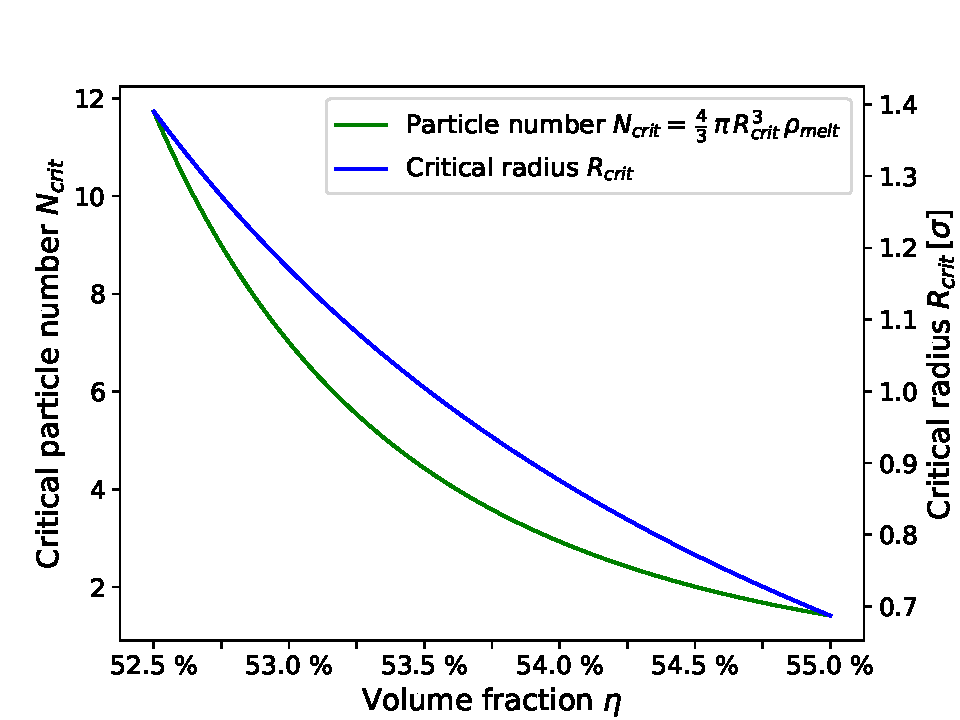
\includegraphics[width=0.7 \linewidth]{CNT_radius.pdf}
\caption{Critical radius $R_{crit}$ calculated from CNT depending on volume fraction $\eta$. As it can be seen the critical radii are rather small. When using the chemical potential calculated by Fillion and Schilling the critical clusters sizes become of the order $N \approx 50$ at intermediate metastable volume fractions, which is much more in agreement with typical largest cluster fluctuations found in simulations. \todo{maybe something is wrong after all with the derivation ?}}
\label{fig:r_crit}
\end{figure}




%To continue in the classical picture an activated process like this is described by a rate given by the Arhenius law:
%\begin{align}
%k&=c \exp{(-\frac{k_B T}{\Delta E})}\\
%\Leftrightarrow \quad k &=c \exp{-\beta \Delta G (R_{crit})}
%\text{\todo{THIS HAS TO BE CORECCTED}}
%\end{align}
%As the constant c is not further defined the absolute nucleation rate in this picture is not predicted but only set into realtion to ther rates. \todo{Check carefully in how far this is correct!}

\section{Memory including approaches}
\label{sec:memory_approach}
CNT assumes a Markovian system, which means that it diffuses through a free energy landscape without granting it memory. But it has been shown by Kuhnbold ... \todo{cite Anjas Lennard-Jones System} that for a Lennard-Jones system memory effects can not be neglected if an accurate  description is desired. Such it must be assumed that also for the Hard Sphere system memory effects may be present.\\

To analyze such memory effects a framework by Hugues Meyer(\todo{cite Hugues}) has been elaborated. In it a memory kernel for coarse-grained observables by means of projection operators is defined together with an efficient algorithm to calculate such.\\
With the derived memory kernel an equation of motion for the observable can be derived, resembling mostly the Generalized Langevin equation is called non-stationary Generalized Langevin Equation because the memory kernel can depend not only on $K(t-\tau)$ but instead on two times $K(t,\tau)$:

\begin{equation}
\label{eqn:EOM_A}
  \frac{d A_{t}}{dt} = \omega (t) A_{t} + \int_{0}^{t} d\tau  K(\tau, t) A_{\tau} + \eta_{t} \quad ,
\end{equation}

For the Markovian process the memory kernel is approximately given by a Dirac delta functional $\delta(\tau-t)$, in which case the Langevin equation is recovered.


\section{Computer Precision}
\label{sec:precision}
%Explain a little about what numerics does, compared to the real world.\\
%Maybe include the time evolution of minimal changes
The precision of computer certainly influences the outcome of simulations. (\todo{talk with Fabian if he found any papers regarding varying results from varying precision over time})\\
And it should always be kept in mind that the simulation only approximates the real world. Even smallest variations in the last digits of positions, changes the simulation radical after a certain number of steps. This comes by the fact that we face a complex system with chaotic behaviour, which means that even small variations will grow exponentially until the system has nothing in common anymore.  
\todo{Look if you can visualize such an behaviour by}
As it can be seen after x timesteps the two system have radically changed.

\section{Comparison to Real world experiments} 
\label{sec:comparison}
%Compare, regadring the solvent. Esspeically with Hajos finding.//
%Maybe connect it with the Computer precision part, to talk about what the s<ystem is and what the system is not
Since the \todo{1950s ?} people have synthesized hard sphere like systems in the lab. Today a whole zoo of systems is known. All of these system have in common, that the hard spheres are in a bath of a fluid, which surrounds them. This fluids density and optical refractive index should match the density and optical refractive index of the hard spheres to prevent segmentation and to enable optical measurements of the system. \todo{maybe elaborate a little more on why each of the two is necessary}\\

The absence of the bath in simple hard sphere simulations is probably the largest difference to the hard sphere systems in the laboratory. It has been argued that the difference can be circumvented by normalizing with a diffusion length or time, but a discussion on the possibility of hydrodynamic effects changing the behaviour of the lab system compared to simulations is ongoing at the moment.\\ 

For simulations it is much harder to include the bath because it introduces a multiple number of particles, making it very slow to simulate large systems.\\




